% Imported from algorithms/video-editing/README.md
\chapter{视频局部编辑}\label{seedance-m08}
\moduleinfo{M08}{基础方法与机制解释}{\hyperref[src-seedance-1.0]{\texttt{seedance-1.0}}、\hyperref[src-vincie]{\texttt{vincie}}、\hyperref[src-vincie-next]{\texttt{vincie-next}}、\hyperref[src-seedance-2.5-release]{\texttt{seedance-2.5-release}}、\hyperref[src-vincie-code]{\texttt{vincie-code}}、\hyperref[src-ltx-code]{\texttt{ltx-code}}}

从参考支路转到源条件支路：编辑先定义变化与保持，再决定怎样编码和合成。

再把生成改成编辑。要求“第二到第四秒的外套变红，其它不动”，目标已经不只是输出一段相似视频，而是同时规定变化对象、时间与保持范围。若这些关系只留在一句提示里，模型即使改对衣服，也可能顺便改了人脸或背景。这里把这几个量分开写。

\section{时间指令怎样变成帧范围}\label{seedance-m08-ux65f6ux95f4ux6307ux4ee4ux600eux6837ux53d8ux6210ux5e27ux8303ux56f4}

先将指令对应到源视频版本、半开时间区间 \([2,4)\)、目标主体和服装区域。随后把不应变化的脸、姿态、背景和音轨也列出来。这样编辑的未知量与已知条件才各有范围。

固定 24 fps 且时间起点为零时，该区间包含帧号 48 到 95。可变帧率视频则应按真实时间戳选帧，不能只用时间乘平均 fps。还要约定第四秒以后是恢复原色，还是延续编辑后的外观；两者对应不同目标。

\section{为什么需要三种 mask}\label{seedance-m08-ux4e3aux4ec0ux4e48ux9700ux8981ux4e09ux79cd-mask}

不过，像素上画出的区域，进入 VAE 和 DiT 后还是同一组独立位置吗？一般不是。时间压缩、卷积感受野与 patch 会混合邻域信息，所以不能把一个像素 mask 不加区分地沿所有阶段使用。需要分别定义：

{\def\LTcaptype{table} % do not increment counter
\small\setlength{\tabcolsep}{3pt}\renewcommand{\arraystretch}{1.18}
\begin{longtable}[]{@{}
  >{\raggedright\arraybackslash}p{(\linewidth - 2\tabcolsep) * \real{0.2200}}
  >{\raggedright\arraybackslash}p{(\linewidth - 2\tabcolsep) * \real{0.7800}}@{}}
\toprule\noalign{}
\begin{minipage}[b]{\linewidth}\raggedright
mask
\end{minipage} & \begin{minipage}[b]{\linewidth}\raggedright
作用
\end{minipage} \\
\midrule\noalign{}
\endhead
\bottomrule\noalign{}
\endlastfoot
编辑 mask & 用户允许最终改变的区域与时间 \\
上下文 mask & 模型需要读取或重建的邻域 \\
损失 mask & 哪些位置具有有效监督 \\
\end{longtable}
}

因此，模型工作区可以向外扩一些，让它读取边界上下文，交付时再按约定只替换允许区域。若改光照本来就会影响外部阴影，则应先扩大允许变化范围；不能既要求全局物理一致，又禁止外部任何像素变化。

\section{生成式补全与像素保留怎样配合}\label{seedance-m08-ux751fux6210ux5f0fux8865ux5168ux4e0eux50cfux7d20ux4fddux7559ux600eux6837ux914dux5408}

一种做法是以源潜变量、mask 和指令为条件，重新生成工作区，较大语义变化容易表达，但外区也可能漂移、边界可能闪烁。另一种做法只生成局部，随后复用外面的源帧。两者的保持机制不同，下面先看后一种合成关系。

设 \(M\) 为最终编辑权重，合成结果为：

\[
x_{\mathrm{out}}=M\odot x_{\mathrm{generated}}+(1-M)\odot x_{\mathrm{source}}.
\]

这个式子中，\(M=0\) 的不编辑位置直接取源像素，因此不必再要求有损 VAE 无损重建外区。软 mask 可以处理过渡，但发丝、运动模糊、透明材质和前后遮挡仍需另外处理。音轨若要求严格保留，也应复用原采样，并检查混流后是否引入延迟。

\section{编辑监督从哪里来}\label{seedance-m08-ux7f16ux8f91ux76d1ux7763ux4eceux54eaux91ccux6765}

真实视频天然包含外观、姿态和物体状态的变化，可以用于挖掘编辑指令和变化区域。

\begin{figure}
\centering
\pandocbounded{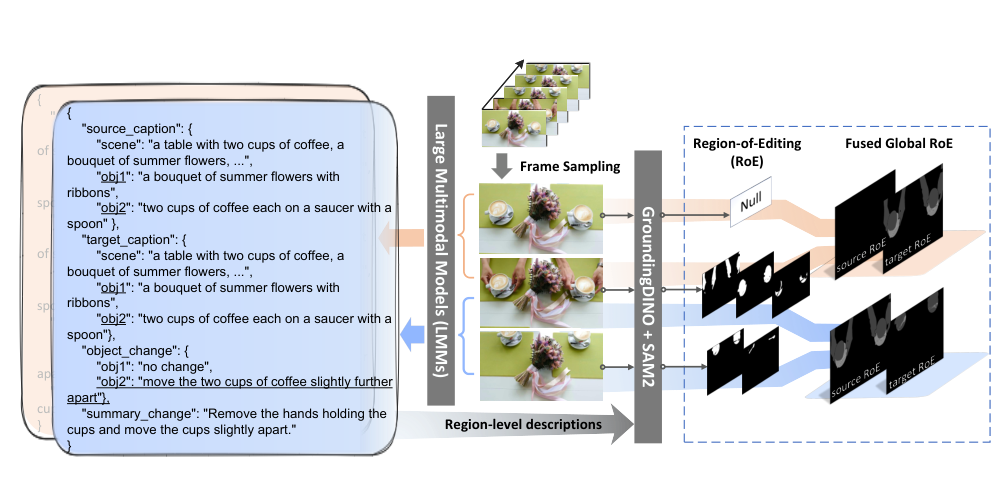
\includegraphics[keepaspectratio,alt={从视频变化构造编辑描述与区域 （论文示意，来源：vincie）}]{assets/seedance/figures/edit-data.png}}
\caption{从视频变化构造编辑描述与区域 （论文示意，来源：vincie）}
\end{figure}

看起来可以从相邻帧直接挖出很多“修改前后对”，但两帧之间可能不止一个因素变化。相机、遮挡、光照都在动，却只标“换衣服颜色”，训练就会把其它变化也学成这条指令的一部分。因此这种配对还不能当作精确单因素真值。

数据来源可以继续分开：受控三维重渲染提供精确几何与 mask；人工真实编辑对记录具体后期操作；视频变化挖掘则作为带置信度的弱监督，并作抽检。三类可以混合使用，但监督的确定程度不能混成一类。

\section{白模与绿幕分别控制什么}\label{seedance-m08-ux767dux6a21ux4e0eux7effux5e55ux5206ux522bux63a7ux5236ux4ec0ux4e48}

白模将布局、相机和运动轨迹先固定，再让生成模型补材质、风格与光照。若同时输出 depth、normal、pose 和相机参数，几何条件更明确；训练时必须保持它们与目标帧严格对齐。由单目视频估计的深度和相机存在误差，需要与精确渲染真值区分。

绿幕编辑先处理 alpha、绿溢色、发丝和运动模糊，再生成背景并做前景光色融合。若还希望衣服受风、头发运动和接触阴影随背景重新变化，任务已经超出单纯抠像，需要重新生成部分前景，并额外验证身份与动作保持。

\section{编辑是否成功，要拆开评价}\label{seedance-m08-ux7f16ux8f91ux662fux5426ux6210ux529fux8981ux62c6ux5f00ux8bc4ux4ef7}

编辑成功怎样看？先确认目标有没有变化，再看非目标有没有保持，接着看时间边界、闪烁、遮挡和音轨。只改颜色可以比较外区像素；改视角时像素本来就变了，应比较身份、语义和几何关系。评价也要随任务定义改变。

编辑并不以 KV 缓存为前提。先用完整重算得到正确结果，再优化哪些依赖可以复用；改动过去内容时，依赖它的后续状态要刷新。最终检查也应覆盖编辑区间前后的帧，不能只挑变化最明显的一张截图。

\section{从极简代码到真实实现}\label{seedance-m08-ux4eceux6781ux7b80ux4ee3ux7801ux5230ux771fux5b9eux5b9eux73b0}

最终保持源像素，只需要明确合成权重；模型内部的工作区和噪声覆盖则是另外两层逻辑：

\begin{verbatim}
selected = (frame_pts >= start) & (frame_pts < end)
output = alpha * generated + (1 - alpha) * source
\end{verbatim}

三种操作的极简代码见 \hyperref[code-local-edit]{local\_edit.py}。真实多轮图像编辑看 \href{https://github.com/ByteDance-Seed/VINCIE/blob/97cd2c5701e694dabcfea320c0cf59893d427fab/generate.py}{VINCIEGenerator}；视频和音视频条件流水线可从 \href{https://github.com/Lightricks/LTX-2/blob/daa6b16fc7f0f1628f2c9e36a303e3312b333cc6/packages/ltx-pipelines/README.md}{LTX pipelines} 选择。VINCIE 的图像编辑入口本身不是时间戳视频编辑器。
